% This is based on the LLNCS.DEM the demonstration file of
% the LaTeX macro package from Springer-Verlag
% for Lecture Notes in Computer Science,
% version 2.4 for LaTeX2e as of 16. April 2010
%
% See http://www.springer.com/computer/lncs/lncs+authors?SGWID=0-40209-0-0-0
% for the full guidelines.
%
\documentclass{article}
\usepackage{amsmath,amssymb}
\usepackage[dvipdfmx]{graphicx}
\usepackage{mediabb}
\usepackage{ascmac}
\begin{document}

\title{MatcherNet: a modular implementation of predictive coding system}
\author{Shigeyuki Oba}

%
% \titlerunning{BundleNet}  % abbreviated title (for running head)
%                                     also used for the TOC unless
%                                     \toctitle is used
%
%\author{Shigeyuki Oba\inst{1} \and Koichi Takahashi\inst{2}}
%
% \authorrunning{Shigeyuki Oba et al.} % abbreviated author list (for running head)
%
%%%% list of authors for the TOC (use if author list has to be modified)
% \tocauthor{Shigeyuki Oba, Koichi Takahashi}
%
%\institute{Kyoto University, Princeton NJ 08544, USA,\\
% \email{oba@i.kyoto-u.ac.jp},\\ WWW home page:
% \texttt{http://ishiilab.jp/}
% \and
% Riken}

\maketitle              % typeset the title of the contribution

\begin{abstract}
Predictive coding is known as a principle to explain information processing in the brain.
Recent extensions of the concept of predictive coding include hierarchical Bayesian modeling of the environment, generation of control signal with active inference, episteminc values for exploration, image translation with deep neural network, etc. 
We propose a general framework that can easily implement a complex model involving multi-modal information processing system with a principled manner.  

%\keywords{predictive coding, model predictive control, artificial general intelligence}
\end{abstract}
%

\newcommand{\vect}[1]{{\bf #1}}
\newcommand{\vA}[0]{\vect{A}}
\newcommand{\vB}[0]{\vect{B}}
\newcommand{\vC}[0]{\vect{C}}
\newcommand{\vF}[0]{\vect{F}}
\newcommand{\vK}[0]{\vect{K}}
\newcommand{\vS}[0]{\vect{S}}
\newcommand{\vQ}[0]{\vect{Q}}
\newcommand{\vR}[0]{\vect{R}}
\newcommand{\T}[0]{{{}^{\rm T}}}
\newcommand{\vu}[0]{\vect{u}}
\newcommand{\vv}[0]{\vect{v}}
\newcommand{\vw}[0]{\vect{w}}
\newcommand{\vx}[0]{\vect{x}}
\newcommand{\vy}[0]{\vect{y}}
\newcommand{\vz}[0]{\vect{z}}
\newcommand{\vmu}{{\boldsymbol{\mu}}}
\newcommand{\vSigma}{{\boldsymbol{\Sigma}}}
\newcommand{\Real}{\mathbb{R}}
\newcommand{\Normal}{{\mathbf{N}}}

\section{Preliminary}
State space models (SSMs) are widely used in order to describe the relationship of stochastic dynamics and noisy observation of the environment. They are used for signal processing, building artificial intelligence to control robots, and mimicking animal behavior. 


\subsection{General SSMs for EKF and its continuous version}
Extended Kalman-filter algorithm is based on a temporary linearization
A state space model assumes a time sequence of latent state variable $\vx_t\in\Real^{N_X}$
behind the observation $\vy_t\in\Real^{N_Y}$ along the discrete time course $t=1,...,T$.


The extended Kalman-filter (EKF) algorithm, in specific, assumes a general model of the following form
\begin{align}
 \vx_{t+1} &= f( \vx_t ) + \vw_t, \\
 \vy_{t} &= g( \vx_t ) + \vz_t
\end{align}
where the two arbitrary differentiable functions
$f(\cdot)$ and $g(\cdot)$ represent the dynamics and observation models, respectively.
$\vw_t$ and $\vz_t$ denote random noise, called system noise and observation noise, obeying the following Gaussian distribution:
\begin{align}
 \vw_{t} \sim N( \vect{0}, \vect{Q} ), \\
 \vz_{t} \sim N( \vect{0}, \vect{R} ).
\end{align}
where $\vect{Q}$ and $\vect{R}$ are covariance matrices of size $N_X\times N_X$ and $N_Y\times N_Y$
representing system noise and observation noise, respectively. 

The goal of the EKF is to approximate the posterior probability of the latent state variable
 $p(\vx_t | \vy_{1:t} )$ as a Gaussian distribution $q_t \equiv q(\vx_t) = N(\vmu_t, \vSigma_t)$,
 with mean $\vmu_t$ and covariance $\vSigma_t$,
 for each time $t=1,\cdots,T$ in an online manner.
 
To this end, a well known sequential algorithm provides a sequential update of the posterior $q_{t+1}$ by only using $q_{t}$ and $\vy_{t+1}$.
In other words, $q_{t}$ brings all the information that was contained in the
past sequence $\vy_{t'}, t'=1,...,t$ so that $q_{t}$ and $\vy_{t+1}$ are sufficient for knowing current update $q_{t+1}$.
The update rule is shown in the Figure \ref{EKFalg}.

We may consider a continuous version of the EKF (cEKF). 
The cEKF assumes a stochastic differential equation, which enables state update with an arbitrary time step $\Delta_t$.
\begin{align}
 \dot\vx  &= f( \vx ) + \vQ d\omega, \label{cont_dyn}\\
 \vy_{t} &= g( \vx_t ) + \vz_t
\end{align}
where $\omega$ denotes a Wiener process such that
$\omega_{t+\Delta t}-\omega_t \sim N(\vect{0},\Delta t\vect{I})$ holds.
The continuous EKF enables arbitrary time step $\Delta t$ such that
 the linear approximation of $f(\cdot)$ holds.
The update algorithm (Figure \ref{EKFalg})
becomes similar to the standard EKF except for the application of the dynamics model.
 
In EKF and cEKF, we may consider $f(\vx)$ and $g(\vx)$ unknown and/or variable. 
They are to be updated in order to decrease the error.

\begin{figure}
%\begin{tabular}{cc}
\begin{itembox}[l]{\bf EKF algorithm}
$(\vmu_{t+1}, \vSigma_{t+1}) \leftarrow (\vmu_t, \vSigma_t)$
\begin{align*}
\vA &\leftarrow \left. \frac{\partial f(\vx)}{\partial \vx} \right|_{\vx = \vmu_t} \\
\bar{\vmu}_t &= \vA \vmu_t \\
\bar{\vSigma}_t &= \vQ + \vA \vSigma_t \vA\T\\ 
\vC &\leftarrow \left. \frac{\partial g(\vx)}{\partial \vx} \right|_{\vx = \vmu_t} \\
\vS &\leftarrow \vR + \vC \bar{\vSigma}_t \vC\T\\
\vK &\leftarrow \bar{\vSigma}_t \vC\T \vS^{-1}\\
\vmu_{t+1} &= \bar{\vmu}_t + \vK \left( \vy-g(\bar{\vmu}_t ) \right)\\
\vSigma_{t+1} &= \bar{\vSigma}_t - \vK \vC \bar{\vSigma}_t
\end{align*}
\end{itembox}

\begin{itembox}[l]{\bf EKF continuous algorithm}
$(\vmu_{t+\Delta t}, \vSigma_{t+\Delta t}) \leftarrow (\vmu_t, \vSigma_t, \Delta t)$
\begin{align*}
\vA &\leftarrow \left. \frac{\partial f(\vx)}{\partial \vx} \right|_{\vx = \vmu_t} \\
\vF &\leftarrow \exp \left( \Delta t \vA \right) \\
\bar{\vmu}_t &= \vF \vmu_t \\
\bar{\vSigma}_t &= \Delta\vQ + \vA \vSigma_t \vA\T\\ 
\vC &\leftarrow \left. \frac{\partial g(\vx)}{\partial \vx} \right|_{\vx = \vmu_t} \\
\vS &\leftarrow \vR + \vC \bar{\vSigma}_t \vC\T\\
\vK &\leftarrow \bar{\vSigma}_t \vC\T \vS^{-1}\\
\vmu_{t+\Delta t} &= \bar{\vmu}_t + \vK \left( \vy-g(\bar{\vmu}_t ) \right)\\
\vSigma_{t+\Delta t} &= \bar{\vSigma}_t - \vK \vC \bar{\vSigma}_t
\end{align*}
\end{itembox}
%\end{tabular}
\caption{EKF algorithms of standard and continuous versions.
Note $\vA, \vF, \vC, \vS, \vK$ are temporal matrices
that are used once at each update of the posterior $q_t$.}
\label{EKFalg}
\end{figure}

%==========================================
\subsection{Multiple inputs and multiple subjects}
We assume multiple input vectors $\vy_m, m=1,\cdots, M$ 
that obey corresponding observation models,
\begin{align}
 \vy_{m} = g_m( \vx ) + \vz_{m} \approx \vC_m \vx + \vz_m
\end{align}
where $g_m(\cdot)$ and $\vC_m$ denotes the $m$-th observation model and its linearized coefficient.
$\vz_m$ is a noise term with Gaussian distribution of covariance $\vR_m$.

We regard a high-dimensional state vector $\vx\in\Real^{D_x}$ as a set of multiple parts of vectors
$\vx=(\vx_1,\cdots,\vx_K)$ where $\vx_k\in\Real^{D_{xk}}, k=1,\cdots, K$.
Then, the dynamics model \eqref{cont_dyn} becomes the following
 multi-part dynamics form without loss of generality:
\begin{align}
 \dot{\vx}_{k} = f_k( \vx ) + \vw_k \approx \sum_{k=1}^K \vA_{kk'} \vx_{k'} + \vw_k
\end{align}
where $f_k(\vx)$ denotes the dynamics model for the $k$th part $\vx_k$ of the state vector $\vx$,
 $\vw_k$ is a system noise term with Gaussian distribution of covariance $\vQ_k$,
 and $\vA_{kk'} \equiv \partial f_k / \partial \vx_{k'}$ is a part of Jacobian matrix corresponding to the $\vx_k$ and $\vx_{k'}$.

We introduce a hidden state vector $\vv\in\Real^{D_v}$ representing an abstract state that can govern
all the original state vectors $\vx_1,\cdots,\vx_K$. Besides, we omit any of the direct interactions among the $K$ state vectors, namely we assume $\vA_{kk'}=\vect{0}$ for $k\neq k'$.
\begin{align}
 \dot{\vx}_{k} =& f_k( \vx, \vv ) + \vw_k \approx  \vA_{kk} \vx_{k} + \vA_{kv} \vv + \vw_k,\\
 \dot{\vv} =& f_v( \vv ) + \vw_v \approx  \vA_{vv} \vv + \vw_v.
\end{align}

\subsection{Hierarchical generalized filter}
The hierarchical generalized filter (GF) is a rich extension to the EKF \cite{GF}.
GF considers a state space models with control signal as a basic building block:
\begin{align*}
s &= g(x,v)+z,& \dot{x} = f(x,v)+w.
\end{align*}
Dynamic system of hidden state variable $x$
is controlled by the control signal $v$
and observed as the sensory signal $s$.
$f()$ and $g()$ are arbitrary function determining
the dynamics model and the observation model, respectively.
$z$ and $w$ are random factors called
observation noise and system noise, respectively.
GF estimates the posterior probability $q(x,v)$
of the sequences of $x,v$ under the given observation sequence of $s$
and a certain prior probability of $v,w$ and $z$.
GF is considered as a recognition system model of human brain \cite{GFGF},
in which $s$ and $x$ called sensory and recognition state
from the context of computational neuroscience.

GF piles up the above state space model 
so that involve hidden states
$x^{(i)}$ and hidden causes $v^{(i)}$, $i=1,...,K$
\cite{Generalized_filter}.
\begin{align}
 \tilde{s} &= \tilde{g}^{(1)}( \tilde{x}^{(1)}, \tilde{v}^{(1)}  ) + \tilde{z}^{(1)},
 &
 \dot{\tilde{x}}^{(1)} = \tilde{f}^{(1)}( \tilde{x}^{(1)}, \tilde{v}^{(1)}  ) + \tilde{w}^{(1)},\\
 \tilde{v}^{(1)} &= \tilde{g}^{(2)}( \tilde{x}^{(2)}, \tilde{v}^{(2)}  ) + \tilde{z}^{(2)},
 &
 \dot{\tilde{x}}^{(2)} = \tilde{f}^{(2)}( \tilde{x}^{(2)}, \tilde{v}^{(2)}  ) + \tilde{w}^{(2)},\\
 \vdots&&&\\
 \tilde{v}^{(i-1)} &= \tilde{g}^{(i)}( \tilde{x}^{(i)}, \tilde{v}^{(i)}  ) + \tilde{z}^{(i)},
 &
 \dot{\tilde{x}}^{(i)} = \tilde{f}^{(i)}( \tilde{x}^{(i)}, \tilde{v}^{(i)}  ) + \tilde{w}^{(i)},\\
 \vdots&&&
\end{align}
It consisted of the following ideas:
\paragraph{Dual expression of internal state}
GF considered the two types of latent variables called hidden state $x$ and hidden cause $v$,
which can be regarded as internal states and control signals in control theory, respectively.
The sensory state (or observation) $s$ is regarded as $v^{(0)}$.
\paragraph{Generalized coordinate}
Each state variable, for example $x^{(1)}$, is
piled up to construct generalized coordinate
 $\tilde{x}^{(1)}=(x^{(1)},\dot{x}^{(1)}, \ddot{x}^{(1)}, ...)$.
$\tilde{s}, \tilde{x}^{(i)}, \tilde{v}^{(i)}$ stands for the same.
$\tilde{f}^{(i)}, \tilde{g}^{(i)},\tilde{z}^{(i)} ,\tilde{w}^{(i)}$.

Here, we consider a simplified expression of the generative model.
Consider the unified latent state $\vu^{(i)} = ( \tilde{x}^{(i)}, \tilde{v}^{(i)})$.
Discretize the generative model 

\begin{figure}[htbp]
  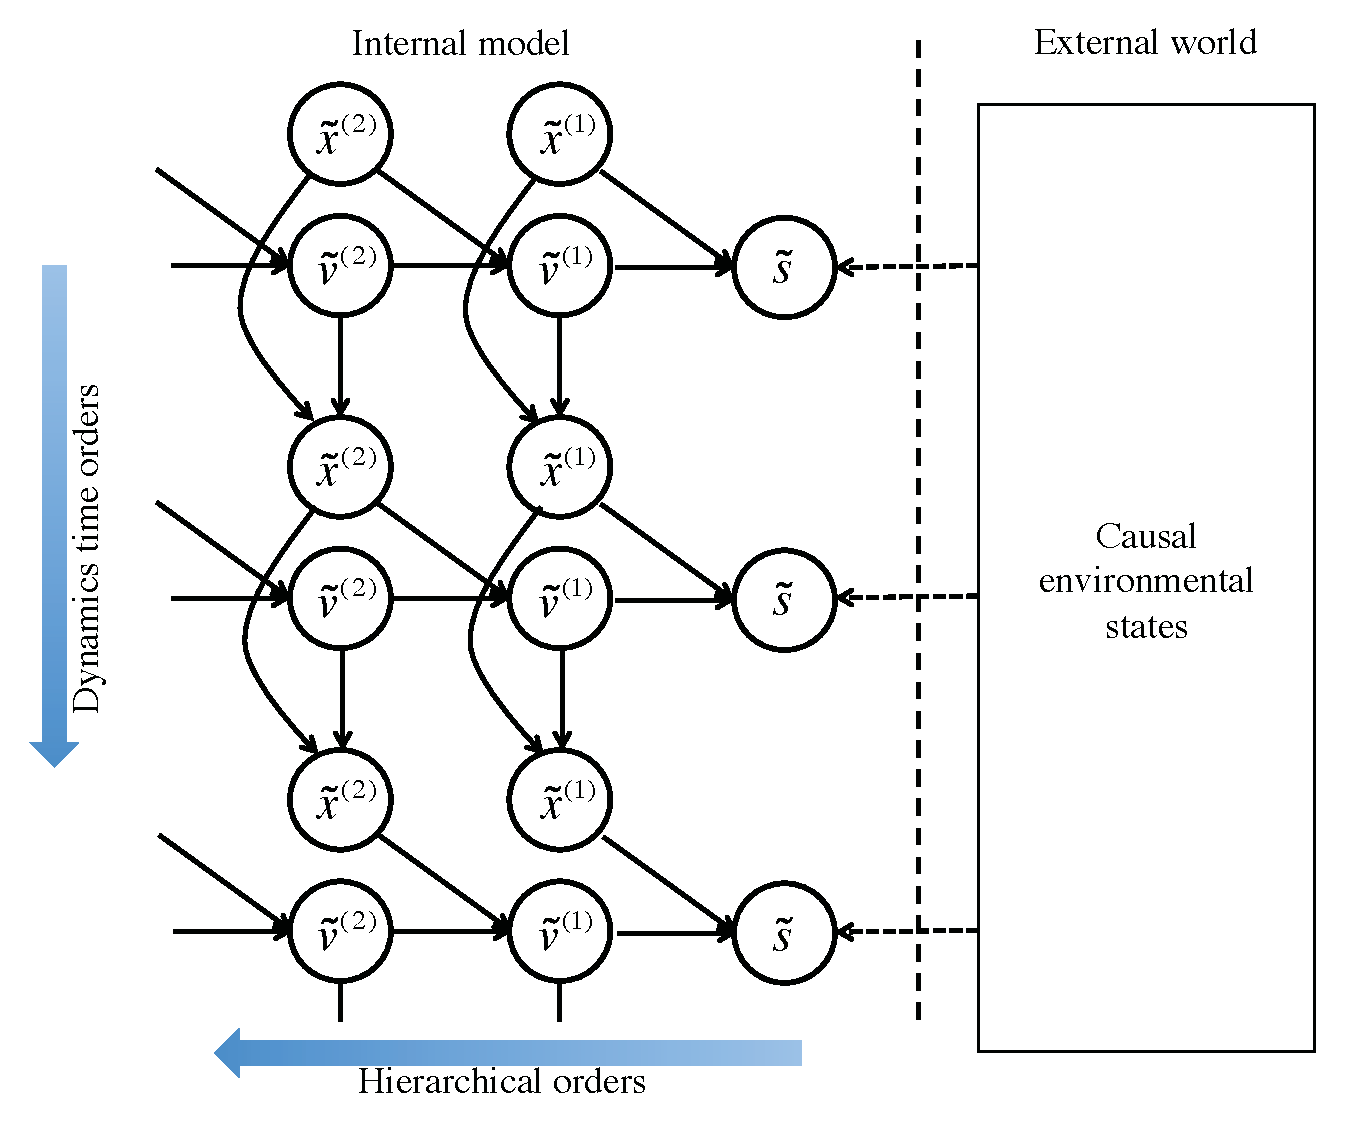
\includegraphics[width=0.8\textwidth]{../figures/gmodel_GF.pdf}
  \caption{Graphical model of the generalized filter. \cite{} }
  \label{g_GF}
\end{figure}
\begin{figure}[htbp]
  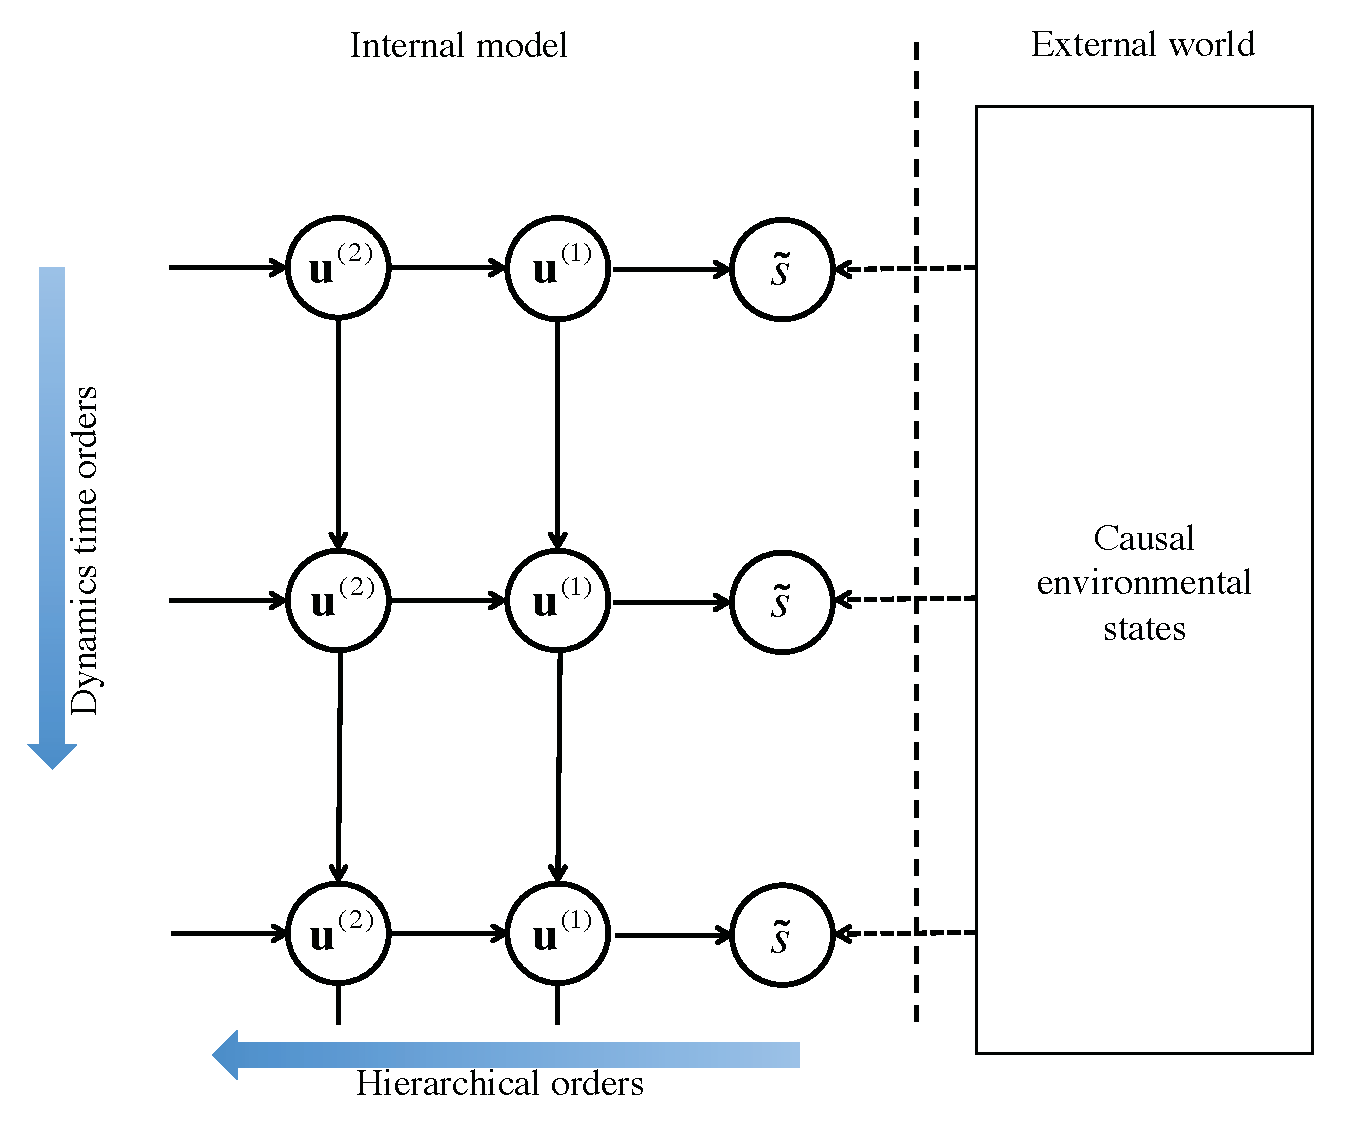
\includegraphics[width=0.8\textwidth]{../figures/gmodel_GF_simple.pdf}
  \caption{A simplified expression. }
  \label{g_GF_simple}
\end{figure}
\begin{figure}[htbp]
  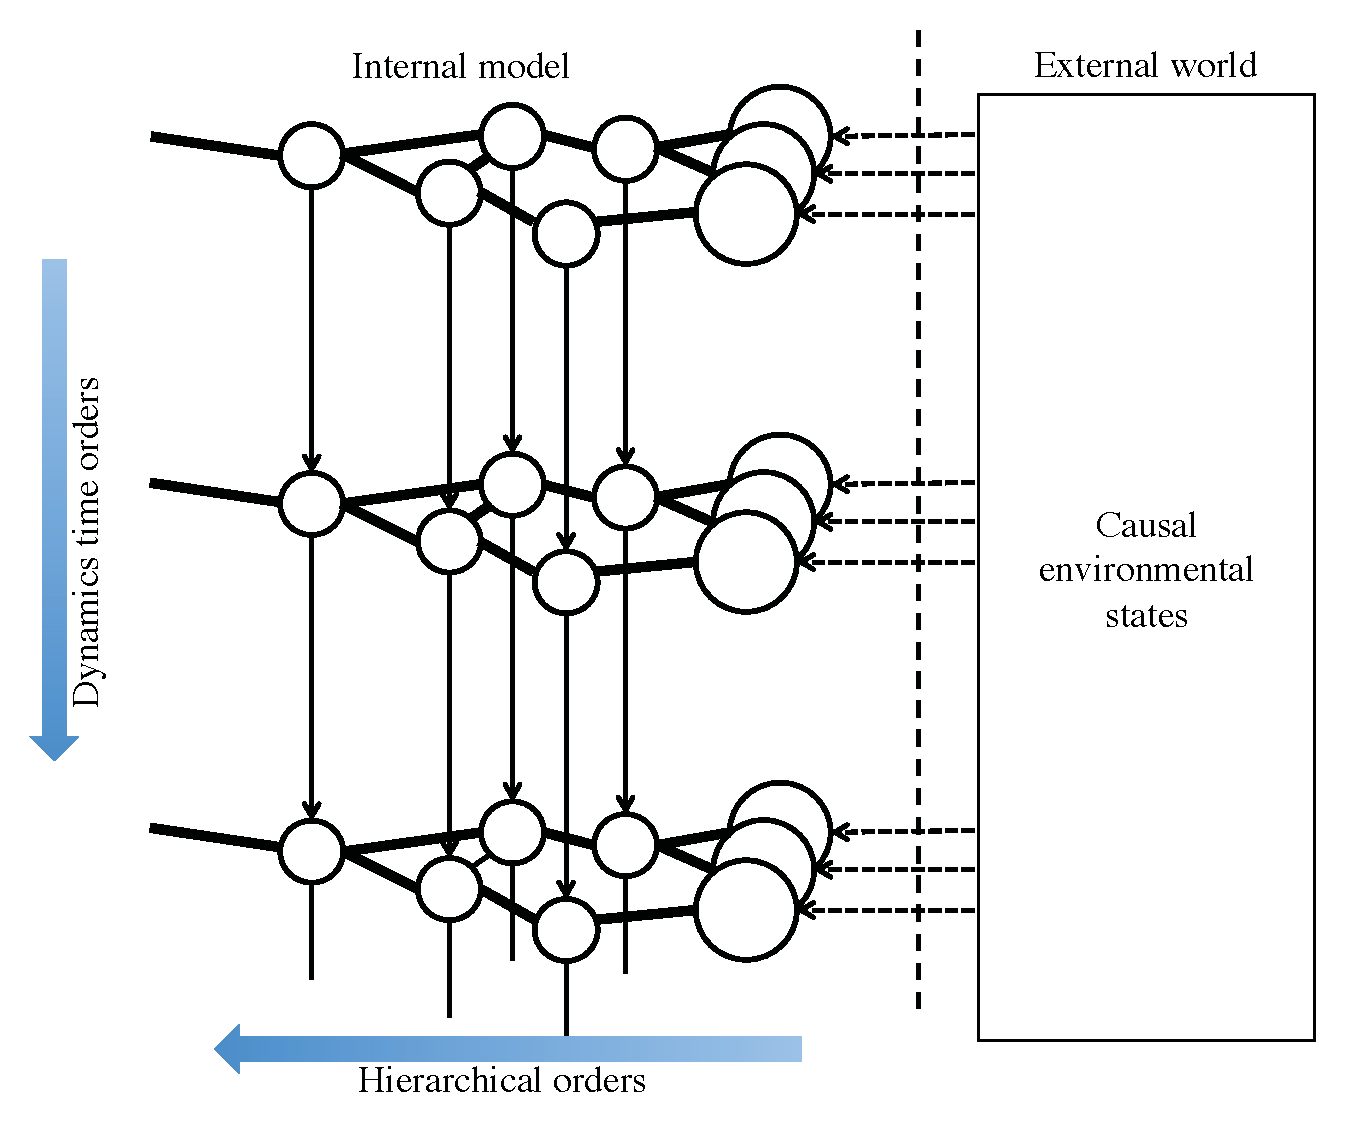
\includegraphics[width=0.8\textwidth]{../figures/gmodel_BN.pdf}
  \caption{Graphical model of bundlenet. 
  White circles connecting each other with thick lines denote
  undirected graph structure of state ing undirected links, connect white circles state nodes, denoted by white circles.
  Vertical directed links connect the state time-point along
   the time order of the internal dynamics model. }
   \label{g_BN}
\end{figure}



\subsection{Free energy principle}
Predictive coding assumes that the internal variable $\vx$ is constructed to predict the observation $\vy$,
which is formulated with a minimization of the following error functional:
\begin{align}
 {\cal E}\{ g(), \vx \} = \sum_t \left|| \vy_{t} - g(\vx_t) \right||^2
\end{align}

$\vx_t$ is determined to predict $\vy_t$ the






\section{Matchernet}
Matchernet is a general framework to build a structured state space modeling of multi-modal signals.

Let us consider a set of three signal sources $\vy_{(1)}, \vy_{(2)}, \vy_{(3)}$ providing
$N_{(1)}, N_{(2)}, N_{(3)}$ dimensional vectors, respectively, in a sequential manner along the time course $t=1, \cdots, T$.
 

Let us consider a set of state variables
$\vx_{(i)} \in \Real^{D_i}, i=1,...,N_B$,
each of which represents a certain aspect of the recognized world.
In robot vision, we may simultaneously consider
left eye vision, right eye vision, their intensity channel, depth channel, higher order visual features,
detected object locations, their motions, recognized categories, etc.
In dynamic brain activity modeling, we may consider activity state of multiple regions of a brain.
Each of $\vx_{(i)}$ has its own dynamical model $p(\vx_{(i), t+1} | \vx_{(i),t} )$
and some, not all, of them has its observation model $p(\vy_{(i),t}|\vx_{(i),t} )$.
Besides, we may consider a relationship model of a set of two or more units of the state,
for example $\vx_{(1)}$ and $\vx_{(2)}$,
which is represented as a joint probability distribution $p(\vx_{(1),t}, \vx_{(2),t} )$.

Since it is a general framework that can represent a large varieties of dynamic models,
we will see some 

We can consider a large and complex dynamics model
 of the total state variable $\vx=(\vx_{(1)}, ..., \vx_{(N_B)})$.


We maintain a probabilistic recognition state $q_i \equiv q( \vx_{(i)} )$ that is a probabilistic distribution of the corresponding part of state vector $\vx_{(i)}$. 


Let  denote the state value vector of the $i$-th model,
$i=1,...,N_B$,
which has its own probabilistic update rule:
\begin{align*}
 p\left( \vx_{(i), t+\Delta t} | \vx_{(i),t}, \theta_{(i)} \right)
\end{align*}

Besides, we assume a joint probability model of a set of states.
\begin{align*}
 p_j\left( \vx_{(1), t}, \vx_{(3), t}, \vx_{(4), t} \right)
\end{align*}



\subsection{EKF as a BundleNet}
EKF is a simple example that is implemented in a BundleNet.

The state update rule of the EKF is divided into the following two steps:
(1) application of the dynamics model and (2) application of the observation model.

(1) dynamics model is applied.
\begin{align*}
\vA &\leftarrow \left. \frac{\partial f(\vx)}{\partial \vx} \right|_{\vx = \vmu_t} \\
\bar{\vmu}_t &= \vA \vmu_t \\
\bar{\vSigma}_t &= \vQ + \vA \vSigma_t \vA\T
\end{align*}

(2) observation model is applied.
\begin{align*}
\vC &\leftarrow \left. \frac{\partial g(\vx)}{\partial \vx} \right|_{\vx = \vmu_t} \\
\vS &\leftarrow \vR + \vC \bar{\vSigma}_t \vC\T\\
\vK &\leftarrow \bar{\vSigma}_t \vC\T \vS^{-1}\\
\vmu_{t+1} &= \bar{\vmu}_t + \vK \left( \vy-g(\bar{\vmu}_t ) \right)\\
\vSigma_{t+1} &= \bar{\vSigma}_t - \vK \vC \bar{\vSigma}_t
\end{align*}


The state $q(\vx)$ consists of mean $\vmu$ and covariance $\vSigma$ 
Here let us regard $\vy$ as an observation of the other state variable 



\subsection{A general formulation of BundleNet}
Bundlenet has a bipartite graph structure connecting two groups of modules, bundles $B_i, i=1,2,...$ and matchers $M_j, j=1,2,...$.
Each bundle 
\subsection{Total Free energy}
The free energy is a sum of all 
\begin{align}
{\cal F} = \sum_{i\in {\cal B}} B_{i} + \sum_{j\in {\cal M}} M_{j}
\end{align}
where ${\cal B}$ and ${\cal M}$ are index sets of all bundles and matchers, respectively.


Each Bundle corresponds to the following term.
\begin{align}
 B_{i} =\langle \ln p( \vx_i(t)|\vx_i(t-1) ) \rangle_{q}
\end{align}

Each Matcher is represented as the following term.
\begin{align}
 M_{j} =\langle \ln p( \epsilon_j ) \rangle_{q}
\end{align}
where $\epsilon_j$ is a function of all the state variables $\vx_i, i\in {\cal B}_{M_j}$.
${\cal B}_{M_j}$ is index of bundles that the matcher $M_j$ links.







\section{Predictive coding and the free energy principle}
Let us make a simple formulation to describe the basic situation involving a recognition system, that is an animal brain for example, living in the real world. Using this simple formulation, we try to tell a simple story of evolution of predictive coding, extension to the Bayesian brain theory, and the free energy principle.

Consider a world model, that is a stochastic state space model involving environmental state ${\bf x}_t$ and its observation ${\bf s}_t$ at time $t$:
\begin{align}
{\bf x}_{t+1} &= {\bf f}({\bf x}_t, {\bf w}_t),\\
{\bf s}_{t} &= {\bf g}({\bf s}_t, {\bf z}_t),
\end{align}
where ${\bf f}()$ and ${\bf g}()$ denotes true environmental dynamics and true perception process that can be stochastic. 
${\bf w}_t$ and ${\bf z}_t$ denotes noise.

On the other hand, we also assume a recognition model, that is also written as a stochastic state space model:
\begin{align}
{x}_{t+1} &= {f}({x}_t, {w}_t),\\
{s}_{t} &= {g}({s}_t, {z}_t),
\end{align}
where $f()$ and $g()$ denotes system dynamics model and noisy observation model for the recognition.

\begin{figure}[hb]
\begin{center}
\begin{tabular}{c|c|c}
& The outer world & Internal recognition \\
\hline
State & ${\bf x}$ & $x$\\
Dynamics & $\dot{\bf x}={\bf f}({\bf x},u)+{\bf z} $ & $\dot{x}=f(x,u)+z $\\
Perception & $s={\bf g}({\bf x})+{\bf w}$ & $s=g(x)+w$ \\
\end{tabular}
\end{center}
\caption{The world and the recognition. Variables/functions that are in the world and not able to directly access from internal recognition are written in bold letters; ${\bf x}, {\bf f}(), {\bf g}()$, etc.}
\end{figure}
Perception $s$\\
Recognition state $x$

Here, let us note some important points, namely, what we assume here and what we do not assume here.
\begin{itemize}
\item Here, we assumed these discrete time expressions for simplicity of the discussion.
Both of the world model and the recognition model are presented as stochastic differential equations in some literatures, \cite{**} Friston's papers.
We assume that these discrete time dynamics are discretized from some continuous time dynamics models. 
\item
There is no guarantee of any synchronization of the time parameter $t$ between the World and Recognition models. Which is an important topic that is to be discussed elsewhere.
\item
Here, we distinguish the recognition state $x_t$ and the true environmental state ${\bf x}_t$. There is no guarantee that they are the same, similar, or having any correspondence. Similarly, there is no guarantee that the system model and the observation model, $f(.)$ and $g(.)$, in the recognition model are the same, similar, or having any correspondence to those in the world model, ${\bf f}()$ and ${\bf g}()$. 
\end{itemize}

\subsection{Predictive coding}
Brain coding theories pursues how the animal brain recognize the environment from its perception.

\subsection{Bayesian brain}

\subsection{Free energy principle}

\section{Bundles and Matchers}
BundleNet consists of several modules
%
With this chapter, the preliminaries are over, and we begin the search
for periodic solutions to Hamiltonian systems. All this will be done in
the convex case; that is, we shall study the boundary-value problem
\begin{eqnarray*}
  \dot{x}&=&JH' (t,x)\\
  x(0) &=& x(T)
\end{eqnarray*}
with $H(t,\cdot)$ a convex function of $x$, going to $+\infty$ when
$\left\|x\right\| \to \infty$.

\subsection{Continuous time extended Kalman filter with BundleNet}
When a state space model with non-linear dynamics is locally linearized, it is locally solved as a Kalman filter. It is called an extended Kalman filter (EKF). Besides, when the non-linear dynamics model is given as a differential equation. We can arbitrarily discretize the time course and obtain continuous time EKF.


%
\begin{thebibliography}{5}
%
\bibitem {clar:eke}
Clarke, F., Ekeland, I.:
Nonlinear oscillations and
boundary-value problems for Hamiltonian systems.
Arch. Rat. Mech. Anal. 78, 315--333 (1982)

\bibitem {clar:eke:2}
Clarke, F., Ekeland, I.:
Solutions p\'{e}riodiques, du
p\'{e}riode donn\'{e}e, des \'{e}quations hamiltoniennes.
Note CRAS Paris 287, 1013--1015 (1978)

\bibitem {mich:tar}
Michalek, R., Tarantello, G.:
Subharmonic solutions with prescribed minimal
period for nonautonomous Hamiltonian systems.
J. Diff. Eq. 72, 28--55 (1988)

\bibitem {rab}
Rabinowitz, P.:
On subharmonic solutions of a Hamiltonian system.
Comm. Pure Appl. Math. 33, 609--633 (1980)

\end{thebibliography}

\end{document}
